%\documentclass{article}
\documentclass[a4paper]{article}\usepackage[]{graphicx}\usepackage[]{xcolor}
% maxwidth is the original width if it is less than linewidth
% otherwise use linewidth (to make sure the graphics do not exceed the margin)
\makeatletter
\def\maxwidth{ %
  \ifdim\Gin@nat@width>\linewidth
    \linewidth
  \else
    \Gin@nat@width
  \fi
}
\makeatother

\definecolor{fgcolor}{rgb}{0.345, 0.345, 0.345}
\newcommand{\hlnum}[1]{\textcolor[rgb]{0.686,0.059,0.569}{#1}}%
\newcommand{\hlstr}[1]{\textcolor[rgb]{0.192,0.494,0.8}{#1}}%
\newcommand{\hlcom}[1]{\textcolor[rgb]{0.678,0.584,0.686}{\textit{#1}}}%
\newcommand{\hlopt}[1]{\textcolor[rgb]{0,0,0}{#1}}%
\newcommand{\hlstd}[1]{\textcolor[rgb]{0.345,0.345,0.345}{#1}}%
\newcommand{\hlkwa}[1]{\textcolor[rgb]{0.161,0.373,0.58}{\textbf{#1}}}%
\newcommand{\hlkwb}[1]{\textcolor[rgb]{0.69,0.353,0.396}{#1}}%
\newcommand{\hlkwc}[1]{\textcolor[rgb]{0.333,0.667,0.333}{#1}}%
\newcommand{\hlkwd}[1]{\textcolor[rgb]{0.737,0.353,0.396}{\textbf{#1}}}%
\let\hlipl\hlkwb

\usepackage{framed}
\makeatletter
\newenvironment{kframe}{%
 \def\at@end@of@kframe{}%
 \ifinner\ifhmode%
  \def\at@end@of@kframe{\end{minipage}}%
  \begin{minipage}{\columnwidth}%
 \fi\fi%
 \def\FrameCommand##1{\hskip\@totalleftmargin \hskip-\fboxsep
 \colorbox{shadecolor}{##1}\hskip-\fboxsep
     % There is no \\@totalrightmargin, so:
     \hskip-\linewidth \hskip-\@totalleftmargin \hskip\columnwidth}%
 \MakeFramed {\advance\hsize-\width
   \@totalleftmargin\z@ \linewidth\hsize
   \@setminipage}}%
 {\par\unskip\endMakeFramed%
 \at@end@of@kframe}
\makeatother

\definecolor{shadecolor}{rgb}{.97, .97, .97}
\definecolor{messagecolor}{rgb}{0, 0, 0}
\definecolor{warningcolor}{rgb}{1, 0, 1}
\definecolor{errorcolor}{rgb}{1, 0, 0}
\newenvironment{knitrout}{}{} % an empty environment to be redefined in TeX

\usepackage{alltt}

\usepackage{hyperref}
\usepackage{float} 
\usepackage{adjustbox}
\usepackage{pdfpages}
\usepackage{xurl}
\usepackage{graphicx}
\usepackage{geometry}
\geometry{verbose,tmargin=3cm,bmargin=3cm,lmargin=3cm,rmargin=1.5cm}




\title{Introduction to R programming: Data preprocessing}
\author{Bernard Silenou$^1$ and Henrik Schanze$^1$}
\date{%
    $^{1}$Department of Epidemiology, Helmholtz Centre for Infection Research, Braunschweig, Germany\\%
   % $^2$Organization 2\\[2ex]%
   \vspace{2em} 
   Version on \today
}
\IfFileExists{upquote.sty}{\usepackage{upquote}}{}
\begin{document}

\maketitle
\vfill
\tableofcontents
\clearpage



\noindent Welcome to this R course on preparing data for analysis (data preprocessing). Before proceeding with this course we recommend that you to get familiar with R-Studio (or what ever IDE you are using) and the content covered in the first chapter of the course titled "Basic R".

\section{Loading packages and data into R}
\subsection*{Goals}
\begin{itemize}
\item Install and load packages
\item Import data into  R
\end{itemize} 

\subsection{Loading packages}
Before loading a package to  your current R session, the package needs to already be installed to your computer. Use the command \texttt{install.packages} to install a package and \texttt{library} to load a package. The RStudio IDE provides an option to search and install  packages. 

\begin{knitrout}
\definecolor{shadecolor}{rgb}{0.969, 0.969, 0.969}\color{fgcolor}\begin{kframe}
\begin{alltt}
\hlkwd{install.packages}\hlstd{(}\hlstr{"MASS"}\hlstd{)}
\hlkwd{library}\hlstd{(MASS)}
\end{alltt}
\end{kframe}
\end{knitrout}

\noindent The command \texttt{install.packages} would install the needed package from the default R repository called CRAN. If the package that you wish to install in not on CRAN, you would need to search for the repository hosting the package, download the tar.gz file before installing it.

\subsection{Loading data}
\noindent We are starting with loading the data we want to work with into R. Data could be stored in different kinds of formats. For the majority of common formats there are simple solutions to import that data.\\
As an example we want to use a \texttt{.csv} file which stores data about movies including the name, genre, rating and a lot more. We can import the file into R using the function \texttt{read.csv} and give it the name  \texttt{dataMovies}.

% though read.table or other methods
% through Rstudio wizard
\begin{knitrout}
\definecolor{shadecolor}{rgb}{0.969, 0.969, 0.969}\color{fgcolor}\begin{kframe}
\begin{alltt}
\hlkwd{setwd}\hlstd{(}\hlstr{"~/Introduction-to-R-programming/lecture_notebooks"}\hlstd{)}
\hlstd{dataMovies} \hlkwb{<-} \hlkwd{read.csv}\hlstd{(}\hlstr{"./data/movies.csv"}\hlstd{)}
\end{alltt}
\end{kframe}
\end{knitrout}
\noindent \texttt{.} in the file path represents the current working directory and  can be printed using \texttt{getwd()} command.





\section{Cleaning and transforming data}

\begin{center}
 
\includegraphics[width = 0.2\textwidth]{./image/cleaning_data.png}    
\end{center} 

\subsection*{Goals}
After reading this section, you should be able to do th following:
\begin{itemize}
\item Deduplicate a data
\item Manipulate character or numeric variables 
\item Subset a data
\item Transform variables in a data
\item Convert data from wide to long formats and back
\item Sort a data
\item Do a single imputation
\end{itemize} 

% useful links: https://www.questionpro.com/blog/data-wrangling/
\noindent At this point, your data should be successfully loaded to your R session. Since raw data often has much noise or missing values, it is essential to be processed thoroughly and carefully before fitting a model to it. \vspace{1em}

\noindent This section showcase some of the steps (identifying outliers, error records and missing values, duplicates records, etc.) in transforming raw data into informative data for analysis. \vspace{1em}

\subsection{Detecting duplicate records}

\begin{center}
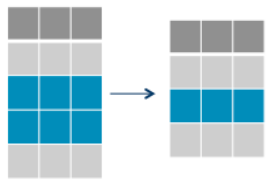
\includegraphics[width = 0.2\textwidth]{./image/deduplication.png}    
\end{center} 
\noindent Duplicate data is in reference to all or a particular variable, often the ID \vspace{1em}

\noindent \textbf{Example:} Identify and remove rows having the same actors \texttt{name} in \texttt{dataMovies} \vspace{1em} 

\begin{knitrout}
\definecolor{shadecolor}{rgb}{0.969, 0.969, 0.969}\color{fgcolor}\begin{kframe}
\begin{alltt}
\hlcom{# checking if there are duplicates}
\hlstd{dataName} \hlkwb{<-} \hlkwd{data.frame}\hlstd{(}\hlkwd{table}\hlstd{(dataMovies}\hlopt{$}\hlstd{name))}
\hlstd{duplicateNames} \hlkwb{<-} \hlstd{dataName[dataName}\hlopt{$}\hlstd{Freq} \hlopt{>}\hlnum{1}\hlstd{,]}
\hlkwd{dim}\hlstd{(duplicateNames)}
\end{alltt}
\begin{verbatim}
## [1] 149   2
\end{verbatim}
\begin{alltt}
\hlkwd{View}\hlstd{(dataMovies[dataMovies}\hlopt{$}\hlstd{name} \hlopt{==} \hlstr{"Anna"}\hlstd{,])}

\hlcom{# Deleting rows with duplicate names at random}
\hlkwd{library}\hlstd{(dplyr)}
\hlstd{dataMoviesDistinctName} \hlkwb{<-} \hlstd{dplyr}\hlopt{::}\hlkwd{distinct}\hlstd{(dataMovies, name,} \hlkwc{.keep_all} \hlstd{=} \hlnum{TRUE}\hlstd{)}

\hlcom{# Deleting rows with duplicate year and score}
\hlstd{dataMoviesDistinctYearScore} \hlkwb{<-} \hlstd{dplyr}\hlopt{::}\hlkwd{distinct}\hlstd{(dataMovies, year, score,} \hlkwc{.keep_all} \hlstd{=} \hlnum{TRUE}\hlstd{)}

\hlcom{# Deleting rows with duplicates for all the columns}
\hlstd{dataMoviesDistinctAll} \hlkwb{<-} \hlstd{dplyr}\hlopt{::}\hlkwd{distinct}\hlstd{(dataMovies,} \hlkwc{.keep_all} \hlstd{=} \hlnum{TRUE}\hlstd{)}
\hlkwd{nrow}\hlstd{(dataMoviesDistinctAll)} \hlcom{# The same as dataMovies}
\end{alltt}
\begin{verbatim}
## [1] 7668
\end{verbatim}
\end{kframe}
\end{knitrout}
%%---------------------------------

\subsection{Adding and deleting colums in a dataframe}

\begin{center}
 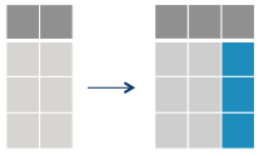
\includegraphics[width = 0.2\textwidth]{./image/adding_column.png}    
\end{center} 

\noindent \textbf{Example:} Compute new variables, for for the total score and another for how old a movie is.\vspace{1em} 

\begin{knitrout}
\definecolor{shadecolor}{rgb}{0.969, 0.969, 0.969}\color{fgcolor}\begin{kframe}
\begin{alltt}
\hlstd{dataMovies}\hlopt{$}\hlstd{age}  \hlkwb{<-} \hlstd{dataMovies}\hlopt{$}\hlstd{yearCurrent} \hlopt{-} \hlstd{dataMovies}\hlopt{$}\hlstd{year}
\hlstd{dataMovies}\hlopt{$}\hlstd{scoreTotal}  \hlkwb{<-} \hlstd{dataMovies}\hlopt{$}\hlstd{score} \hlopt{+} \hlstd{dataMovies}\hlopt{$}\hlstd{scoreSecond}
\hlkwd{head}\hlstd{(dataMovies,} \hlnum{3}\hlstd{)[,} \hlkwd{c}\hlstd{(}\hlnum{1}\hlstd{,}\hlnum{20}\hlopt{:}\hlkwd{ncol}\hlstd{(dataMovies))]}
\end{alltt}
\begin{verbatim}
##                                             name age scoreTotal
## 1                                    The Shining  43   18.80959
## 2                                The Blue Lagoon  43   11.00959
## 3 Star Wars: Episode V - The Empire Strikes Back  43   19.70959
\end{verbatim}
\end{kframe}
\end{knitrout}
\noindent Using the the command \texttt{within} reduces typing effort and leads to clean code.
\begin{knitrout}
\definecolor{shadecolor}{rgb}{0.969, 0.969, 0.969}\color{fgcolor}\begin{kframe}
\begin{alltt}
\hlstd{dataMovies} \hlkwb{<-} \hlkwd{within}\hlstd{(}
\hlkwc{data} \hlstd{= dataMovies,}
\hlkwc{expr} \hlstd{= \{}
\hlstd{age} \hlkwb{=} \hlstd{yearCurrent} \hlopt{-} \hlstd{year}
\hlstd{scoreTotal}  \hlkwb{=} \hlstd{score} \hlopt{+} \hlstd{scoreSecond}
\hlstd{movies21Century} \hlkwb{=} \hlstd{year} \hlopt{>} \hlnum{2000}
\hlstd{\}}
\hlstd{)}
\end{alltt}
\end{kframe}
\end{knitrout}

\noindent \textbf{Quick exercise:} 
\begin{enumerate}
\item Extract the data call dataMoviesNegativeScore for movies with negative second score (scoreSecond) from dataMovies. Which movie has the smallest score and which has the maximum score.
\end{enumerate}

%%---------------------------------
\subsection{Cleaning character variables}
Data values can be recorded in a way that R does not understand, for example, a question that requires a TRUE or FALSE response may have been recorded as \textit{Y} or \textit{N},  or \textit{Yes} or \textit{No}. \vspace{1em} \\ 
\noindent \textbf{Example:} \vspace{1em} 

\noindent Replace the character variable \textit{drugUse} with the logical value \textit{TRUE} or \textit{FALSE}.
\begin{knitrout}
\definecolor{shadecolor}{rgb}{0.969, 0.969, 0.969}\color{fgcolor}\begin{kframe}
\begin{alltt}
\hlstd{characterToLogical} \hlkwb{<-} \hlkwa{function}\hlstd{(}\hlkwc{x}\hlstd{)\{}
\hlstd{n} \hlkwb{=} \hlkwd{length}\hlstd{(x)}
\hlstd{y} \hlkwb{=} \hlkwd{rep}\hlstd{(}\hlnum{NA}\hlstd{, n)}
\hlstd{y[x} \hlopt{==} \hlstr{"Yes"}\hlstd{]} \hlkwb{=} \hlnum{TRUE}
\hlstd{y[x} \hlopt{==} \hlstr{"No"}\hlstd{]} \hlkwb{<-} \hlnum{FALSE}
\hlkwd{return}\hlstd{(y)}
\hlstd{\}}
\hlstd{dataMovies}\hlopt{$}\hlstd{drugUseLogical} \hlkwb{=} \hlstd{(}\hlkwd{characterToLogical}\hlstd{(dataMovies}\hlopt{$}\hlstd{drugUse))}
\end{alltt}
\end{kframe}
\end{knitrout}

\noindent Have a look at the sex of the director \texttt{sexDirector} and code males with \texttt{Male} and famales with \texttt{Female}. 

\begin{knitrout}
\definecolor{shadecolor}{rgb}{0.969, 0.969, 0.969}\color{fgcolor}\begin{kframe}
\begin{alltt}
\hlkwd{table}\hlstd{(dataMovies}\hlopt{$}\hlstd{sexDirector,} \hlkwc{useNA} \hlstd{=} \hlstr{"always"}\hlstd{)} \hlcom{# always, to display missing values}
\end{alltt}
\begin{verbatim}
## 
##      f Female      M   male   Male   <NA> 
##   1221   1324   1311   1229   1277   1306
\end{verbatim}
\begin{alltt}
\hlstd{replacing_enums} \hlkwb{<-} \hlkwa{function}\hlstd{(}\hlkwc{x}\hlstd{)\{}
\hlstd{n} \hlkwb{=} \hlkwd{length}\hlstd{(x)}
\hlstd{y} \hlkwb{=} \hlkwd{rep}\hlstd{(}\hlnum{NA}\hlstd{, n)}
\hlstd{y[x} \hlopt \hlkwd{c}\hlstd{(}\hlstr{"f"}\hlstd{,} \hlstr{"Female"}\hlstd{)]} \hlkwb{=} \hlstr{"Female"} \hlcom{# %in% to check for multiple options}
\hlstd{y[x} \hlopt \hlkwd{c}\hlstd{(}\hlstr{"M"}\hlstd{,} \hlstr{"male"}\hlstd{,} \hlstr{"Male"}\hlstd{)]} \hlkwb{=} \hlstr{"Male"}
\hlkwd{return}\hlstd{(y)}
\hlstd{\}}
\hlstd{dataMovies}\hlopt{$}\hlstd{sexDirectorClean} \hlkwb{=} \hlstd{(}\hlkwd{replacing_enums}\hlstd{(dataMovies}\hlopt{$}\hlstd{sexDirector))}
\end{alltt}
\end{kframe}
\end{knitrout}

\noindent \textbf{Quick exercise:} Create a dummy (indicator) variable call drugUseDummy for drugUse. Code Yes with 1 and No with 0. What is the data type of drugUseDummy?

%%---------------------------------
\subsection{Cleaning numeric variables}
Data values can be recorded with \textit{errors}. For example, age of 114 yrs for a person. This age value may not be an error but doesn't belong to the population that we are interested in (\textit{outlier}) \vspace{1em}

\noindent We want to identify and either correct the age of the person (if its an error record) or drop the person from the study (outlier). \vspace{1em}


\noindent \textbf{Example:}  Assume the required age is between 10 and 40 yrs.  \vspace{1em}

\noindent Are there records having an \texttt{age} that is not between 10 and 40 yrs? If Yes, how many? \vspace{1em}

\noindent Create a new data set having only records with \texttt{age} between 10 and 40 yrs \vspace{1em}

\noindent Replace all records having age below 10 years with 10yrs and those above 40yrs with 40yrs \vspace{1em}


\begin{knitrout}
\definecolor{shadecolor}{rgb}{0.969, 0.969, 0.969}\color{fgcolor}\begin{kframe}
\begin{alltt}
\hlkwd{table}\hlstd{(}\hlkwd{is.na}\hlstd{(dataMovies}\hlopt{$}\hlstd{age))} \hlcom{# checking for missing data}
\end{alltt}
\begin{verbatim}
## 
## FALSE 
##  7668
\end{verbatim}
\begin{alltt}
\hlkwd{summary}\hlstd{(dataMovies}\hlopt{$}\hlstd{age)} \hlcom{# Summary of age }
\end{alltt}
\begin{verbatim}
##    Min. 1st Qu.  Median    Mean 3rd Qu.    Max. 
##    3.00   13.00   23.00   22.59   32.00   43.00
\end{verbatim}
\begin{alltt}
\hlcom{# Filtering records with age less than 10 or grater than 40}
\hlstd{dataMoviesAgeNot10to40} \hlkwb{<-} \hlstd{dataMovies[(dataMovies}\hlopt{$}\hlstd{age} \hlopt{<} \hlnum{10} \hlopt{|} \hlstd{dataMovies}\hlopt{$}\hlstd{age} \hlopt{>} \hlnum{40}\hlstd{), ]}
\hlcom{#Counting number of records}
\hlkwd{nrow}\hlstd{(dataMoviesAgeNot10to40)} \hlcom{# or dim(dataMoviesAgeNot10to40)[1]}
\end{alltt}
\begin{verbatim}
## [1] 1556
\end{verbatim}
\begin{alltt}
\hlcom{# Alternately, we can negate the condition to filter for age between 10 to 40}
\hlstd{dataMoviesAge10to40} \hlkwb{<-} \hlstd{dataMovies[}\hlopt{!}\hlstd{(dataMovies}\hlopt{$}\hlstd{age} \hlopt{<} \hlnum{10} \hlopt{|} \hlstd{dataMovies}\hlopt{$}\hlstd{age} \hlopt{>} \hlnum{40}\hlstd{), ]}
\hlcom{# OR }
\hlstd{dataMoviesAge10to40} \hlkwb{<-} \hlstd{dataMovies[(dataMovies}\hlopt{$}\hlstd{age} \hlopt{>=} \hlnum{10} \hlopt{&} \hlstd{dataMovies}\hlopt{$}\hlstd{age} \hlopt{<=} \hlnum{40}\hlstd{), ]}

\hlcom{# Replacing numeric variables}
\hlcom{# Copying age to a new column called ageImputed }
\hlcom{# It is not advisable to manipulate existing variables}
\hlstd{dataMovies}\hlopt{$}\hlstd{ageImputed} \hlkwb{<-} \hlstd{dataMovies}\hlopt{$}\hlstd{age}
\hlcom{# Replacing ages less than 10 with 10}
\hlstd{dataMovies}\hlopt{$}\hlstd{ageImputed[dataMovies}\hlopt{$}\hlstd{ageImputed} \hlopt{<} \hlnum{10}\hlstd{]} \hlkwb{<-} \hlnum{10}
\hlcom{# Replacing ages greater than 40 with 40}
\hlstd{dataMovies}\hlopt{$}\hlstd{ageImputed[dataMovies}\hlopt{$}\hlstd{ageImputed} \hlopt{>} \hlnum{40}\hlstd{]} \hlkwb{<-} \hlnum{40}  \hlcom{# do this same task using within function}
\end{alltt}
\end{kframe}
\end{knitrout}

\noindent \textbf{Homework:} Write a function that compute the median \texttt{score} and assign its value to all records having missing values for \texttt{score}.

%%---------------------------------

\subsection{Sorting}

\begin{center}

\includegraphics[width = 0.2\textwidth]{./image/sorting.png}    
\end{center} 

\noindent Sorting involves \textit{arranging} data into some  \textit{meaningful order} to make it easier to understand or analyse. \vspace{1em}

\noindent \textbf{Example:} Sort \texttt{dataMovies} using the following variables: (a) \texttt{year} , (b) \texttt{rating} , (c) \texttt{score} and \texttt{votes}. 

\begin{knitrout}
\definecolor{shadecolor}{rgb}{0.969, 0.969, 0.969}\color{fgcolor}\begin{kframe}
\begin{alltt}
\hlcom{# Sorting by year (integer)}
\hlstd{dataMoviesSortYear} \hlkwb{<-}  \hlstd{dataMovies[}\hlkwd{order}\hlstd{(dataMovies}\hlopt{$}\hlstd{year), ]}
\hlcom{# Use the general form "vector[order(vector)]" # to sort a vector}

\hlcom{# Sorting by rating (character)}
\hlstd{dataMoviesSortRating} \hlkwb{<-}  \hlstd{dataMovies[}\hlkwd{order}\hlstd{(dataMovies}\hlopt{$}\hlstd{rating,} \hlkwc{decreasing} \hlstd{= T), ]}

\hlcom{# Sorting by score (numeric) and rating (character), Order matters!}
\hlstd{dataMoviesSortScoreRating} \hlkwb{=}  \hlstd{dataMovies[}\hlkwd{order}\hlstd{(dataMovies}\hlopt{$}\hlstd{score, dataMovies}\hlopt{$}\hlstd{rating), ]}
\hlcom{# OR using the "with" command}
\hlstd{dataMoviesSortScoreRatingWith} \hlkwb{=} \hlstd{dataMovies[}\hlkwd{with}\hlstd{(dataMovies,} \hlkwd{order}\hlstd{(score, rating)), ]}
\end{alltt}
\end{kframe}
\end{knitrout}
  
\noindent \textbf{Quick exercise:} \vspace{1em}

\noindent (a) Sort \texttt{dataMovies} using variables \texttt{score} and \texttt{writer}.  \vspace{1em}

\noindent (b) Would you have the same results if you sort by: (i) \texttt{writer} and  \texttt{score},  (ii) First by \texttt{score} only and then by \texttt{writer} only?

%%---------------------------------
\subsection{Converting between wide and long form}

\begin{center}
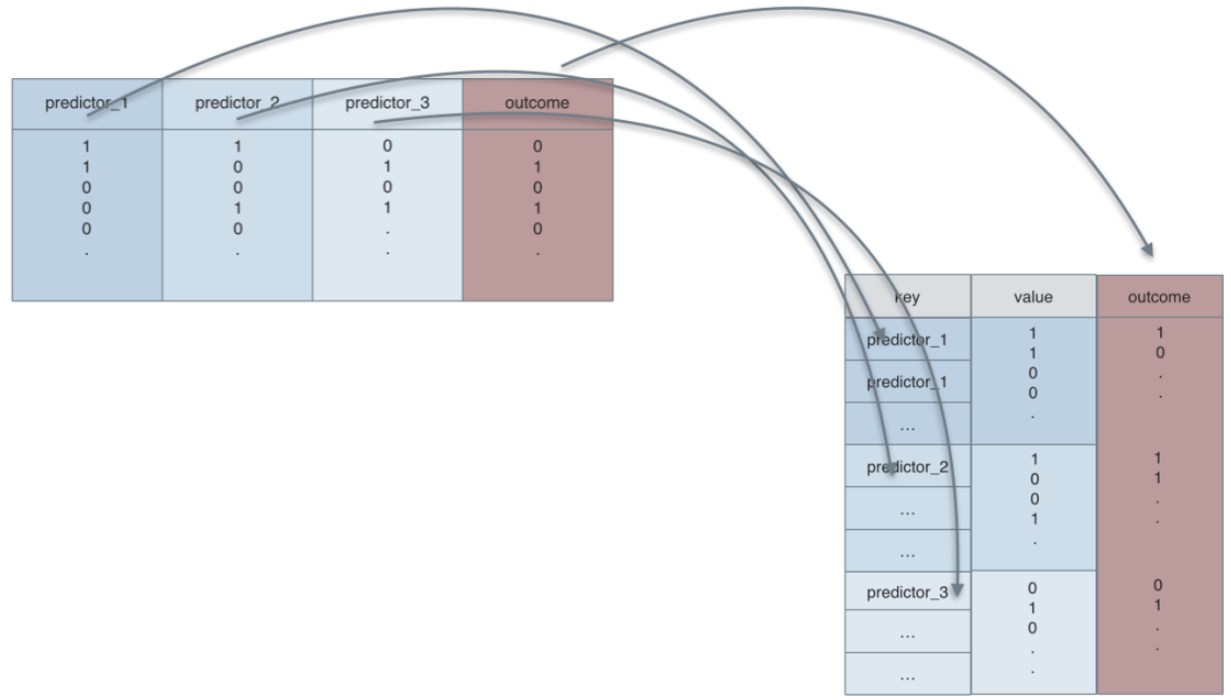
\includegraphics[width = 0.7\textwidth]{./image/wide_long_format.png}    
\end{center} 

\noindent Wide format: a single row for every data point and multiple columns for the varables or predictors. \vspace{1em} \\
Long format: for each data point there are many rows as the number of variables.    \vspace{1em} 

\noindent The \texttt{melt} function in the \texttt{reshape2} package converts from wide to long. The \texttt{dcast} function does the opposite. \vspace{1em}

\noindent All the variables or predictors should be of the \textit{same data type} \vspace{1em}

\noindent \textbf{Example:} Convert \texttt{dataMovies} data to long format and back to wide format.


\begin{knitrout}
\definecolor{shadecolor}{rgb}{0.969, 0.969, 0.969}\color{fgcolor}\begin{kframe}
\begin{alltt}
\hlkwd{library}\hlstd{(reshape2)}
\hlcom{# Converting from wide to long format}
\hlstd{dataMoviesScoresGross} \hlkwb{<-} \hlstd{dataMovies[,} \hlkwd{colnames}\hlstd{(dataMovies)} \hlopt
                                     \hlkwd{c}\hlstd{(}\hlstr{"name"}\hlstd{,} \hlstr{"score"}\hlstd{,} \hlstr{"scoreSecond"}\hlstd{,}  \hlstr{"gross"}\hlstd{)]}
\hlstd{dataMoviesScoresGrossLong} \hlkwb{=} \hlkwd{melt}\hlstd{(}\hlkwc{data} \hlstd{= dataMoviesScoresGross,} \hlkwc{id.vars} \hlstd{=} \hlstr{"name"}\hlstd{)}

\hlstd{dataMoviesSortScoreRatingWith} \hlkwb{=} \hlstd{dataMovies[}\hlkwd{with}\hlstd{(dataMovies,} \hlkwd{order}\hlstd{(score, rating)), ]}


\hlkwd{head}\hlstd{(dataMoviesScoresGrossLong[}\hlkwd{with}\hlstd{(dataMoviesScoresGrossLong,} \hlkwd{order}\hlstd{(name)),],} \hlnum{10}\hlstd{)}
\end{alltt}
\begin{verbatim}
##                  name    variable        value
## 6570              '71       score 7.200000e+00
## 14238             '71       gross 3.062178e+06
## 21906             '71 scoreSecond 8.009589e+00
## 1014   'night, Mother       score 7.600000e+00
## 8682   'night, Mother       gross 4.418630e+05
## 16350  'night, Mother scoreSecond 8.809589e+00
## 1007  'Round Midnight       score 7.400000e+00
## 8675  'Round Midnight       gross 3.272593e+06
## 16343 'Round Midnight scoreSecond 8.409589e+00
## 5643           [Rec]²       score 6.500000e+00
\end{verbatim}
\begin{alltt}
\hlcom{# Converting from long to wide format}
\hlcom{#deer_wide_again <- reshape2::dcast(deer_long, SkullID ~ variable)}
\hlstd{dataMoviesScoresGrossWide} \hlkwb{<-} \hlstd{reshape2}\hlopt{::}\hlkwd{dcast}\hlstd{(}\hlkwc{data} \hlstd{= dataMoviesScoresGrossLong,}
                                            \hlkwc{value.var}\hlstd{=}\hlstr{"value"}\hlstd{, mean,} \hlkwc{formula} \hlstd{= name} \hlopt{~} \hlstd{variable)}
\end{alltt}
\end{kframe}
\end{knitrout}

%\noindent \textbf{Quick exercise:} 
%%---------------------------------

\subsection{Detecting missing values}
\begin{center}

\includegraphics[width = 0.25\textwidth]{./image/missing_values.png}    
\end{center} 

\noindent Missing data, or missing values, occur when no data value is stored for a variable in an observation. Missing data are coded as \texttt{NA} in R.\vspace{1em} 

\noindent \textbf{Example 1:} \\
\noindent How many movies have missing data for the directors' sex (\texttt{sexDirectorClean})? \\
\noindent How many movies have complete data for all the variables (columns)? \vspace{1em} 

\begin{knitrout}
\definecolor{shadecolor}{rgb}{0.969, 0.969, 0.969}\color{fgcolor}\begin{kframe}
\begin{alltt}
\hlcom{# Counting the number of categories, including NA}
\hlkwd{table}\hlstd{(dataMovies}\hlopt{$}\hlstd{sexDirectorClean,} \hlkwc{useNA} \hlstd{=} \hlstr{"always"}\hlstd{)}
\end{alltt}
\begin{verbatim}
## 
## Female   Male   <NA> 
##   2545   3817   1306
\end{verbatim}
\begin{alltt}
\hlcom{# Extracting data with complete cases across the entire columns}
\hlstd{has_all_measurements} \hlkwb{<-} \hlkwd{complete.cases}\hlstd{(dataMovies)}
\hlstd{dataMoviesComplete} \hlkwb{<-} \hlstd{dataMovies[has_all_measurements, ]}
\hlcom{# dataMovies[has_all_measurements, ] is the same as dataMovies[has_all_measurements==TRUE, ]}
\hlcom{# dataMoviesComplete = na.omit(dataMovies) # does the same job}

\hlcom{# Extracting data with at least one incomplete case across the entire columns}
\hlstd{dataMoviesIncomplete} \hlkwb{<-} \hlstd{dataMovies[has_all_measurements} \hlopt{==} \hlnum{FALSE}\hlstd{, ]}
\end{alltt}
\end{kframe}
\end{knitrout}

\noindent How can we address missing values in our analysis? A statistical method called Multiple Imputation (MI) can be used. MI is beyond the scope of this course. However, the  \href{https://cran.r-project.org/web/packages/mice/index.html}{mice}  package is a good references to look at if needed. \vspace{1em} 

\noindent \textbf{Example 2:} How many movies have missing \texttt{score}. Remember that \texttt{score} is a numeric vector. Create a data set called  \texttt{dataMoviesIncompleteScore} having only records with  missing scores.
\begin{knitrout}
\definecolor{shadecolor}{rgb}{0.969, 0.969, 0.969}\color{fgcolor}\begin{kframe}
\begin{alltt}
\hlcom{# Creating a logical vector for score status (missing or available)}
\hlstd{is_score_missing} \hlkwb{<-} \hlkwd{is.na}\hlstd{(dataMovies}\hlopt{$}\hlstd{score)}
\hlkwd{table}\hlstd{(is_score_missing)}
\end{alltt}
\begin{verbatim}
## is_score_missing
## FALSE  TRUE 
##  7665     3
\end{verbatim}
\begin{alltt}
\hlcom{# Alternative solution}
\hlcom{# summary(dataMovies)}
\hlcom{# summary(dataMovies$score)}

\hlcom{# Creating data with missing scores}
\hlstd{dataMoviesIncompleteScore} \hlkwb{<-} \hlstd{dataMovies[is_score_missing,]}
\hlstd{dataMoviesCompleteScore} \hlkwb{<-} \hlstd{dataMovies[}\hlopt{!}\hlstd{is_score_missing,]}
\end{alltt}
\end{kframe}
\end{knitrout}

\noindent \textbf{Quick exercise:} Create a data excluding missing values for  \texttt{gross} or  \texttt{sexDirector}. Are there records with missing values for  \texttt{budget} and  \texttt{gross}?

\begin{knitrout}
\definecolor{shadecolor}{rgb}{0.969, 0.969, 0.969}\color{fgcolor}\begin{kframe}
\begin{alltt}
\hlstd{condition} \hlkwb{<-} \hlkwd{with}\hlstd{(}\hlkwc{data} \hlstd{= dataMovies,} \hlkwc{expr} \hlstd{= (}\hlkwd{is.na}\hlstd{(gross)} \hlopt{|} \hlkwd{is.na}\hlstd{(sexDirector)) )}
\hlstd{dataMoviesMissingGrosOrSexDirector} \hlkwb{<-} \hlstd{dataMovies[}\hlopt{!}\hlstd{condition,]}
\end{alltt}
\end{kframe}
\end{knitrout}

\noindent \textbf{Quick Exercise:} A few cells  in the column rating of  \texttt{dataMovies} are empty. Count the number of empty cells and replace them with  \texttt{NA}, the rightful notation.

%%---------------------------------
%\subsection{Merging}

\end{document}
